\documentclass[]{article}
\usepackage[left=1in,top=1in,right=1in,bottom=1in]{geometry}


%%%% more monte %%%%
% thispagestyle{empty}
% https://stackoverflow.com/questions/2166557/how-to-hide-the-page-number-in-latex-on-first-page-of-a-chapter
\usepackage{color}
% \usepackage[table]{xcolor} % are they using color?

% \definecolor{WSU.crimson}{HTML}{981e32}
% \definecolor{WSU.gray}{HTML}{5e6a71}

% \definecolor{shadecolor}{RGB}{248,248,248}
\definecolor{WSU.crimson}{RGB}{152,30,50} % use http://colors.mshaffer.com to convert from 981e32
\definecolor{WSU.gray}{RGB}{94,106,113}

%%%%%%%%%%%%%%%%%%%%%%%%%%%%

\newcommand*{\authorfont}{\fontfamily{phv}\selectfont}
\usepackage{lmodern}


  \usepackage[T1]{fontenc}
  \usepackage[utf8]{inputenc}




\usepackage{abstract}
\renewcommand{\abstractname}{}    % clear the title
\renewcommand{\absnamepos}{empty} % originally center

\renewenvironment{abstract}
 {{%
    \setlength{\leftmargin}{0mm}
    \setlength{\rightmargin}{\leftmargin}%
  }%
  \relax}
 {\endlist}

\makeatletter
\def\@maketitle{%
  \pagestyle{empty}
  \newpage
%  \null
%  \vskip 2em%
%  \begin{center}%
  \let \footnote \thanks
    {\fontsize{18}{20}\selectfont\raggedright  \setlength{\parindent}{0pt} \@title \par}%
}
%\fi
\makeatother









\title{\textbf{\textcolor{WSU.crimson}{Will Smith VS Denzel
Washington}} \newline \textbf{\textcolor{WSU.gray}{Which Actor is
better?}}  }
 

%  

% \author{ \Large true \hfill \normalsize \emph{} }
\author{\Large Nic
Trout\vspace{0.05in} \newline\normalsize\emph{Washington State
University}  }


\date{December 14, 2020}
\setcounter{secnumdepth}{3}

\usepackage{titlesec}
% See the link above: KOMA classes are not compatible with titlesec any more. Sorry.
% https://github.com/jbezos/titlesec/issues/11
\titleformat*{\section}{\bfseries}
\titleformat*{\subsection}{\bfseries\itshape}
\titleformat*{\subsubsection}{\itshape}
\titleformat*{\paragraph}{\itshape}
\titleformat*{\subparagraph}{\itshape}

% https://code.usgs.gov/usgs/norock/irvine_k/ip-092225/


%\titleformat*{\section}{\normalsize\bfseries}
%\titleformat*{\subsection}{\normalsize\itshape}
%\titleformat*{\subsubsection}{\normalsize\itshape}
%\titleformat*{\paragraph}{\normalsize\itshape}
%\titleformat*{\subparagraph}{\normalsize\itshape}

% https://tex.stackexchange.com/questions/233866/one-column-multicol-environment#233904
\usepackage{environ}
\NewEnviron{auxmulticols}[1]{%
  \ifnum#1<2\relax% Fewer than 2 columns
    %\vspace{-\baselineskip}% Possible vertical correction
    \BODY
  \else% More than 1 column
    \begin{multicols}{#1}
      \BODY
    \end{multicols}%
  \fi
}





\usepackage{natbib}
\setcitestyle{aysep={}} %% no year, comma just year
% \usepackage[numbers]{natbib}
\bibliographystyle{./../biblio/ormsv080.bst}



\usepackage[strings]{underscore} % protect underscores in most circumstances




\newtheorem{hypothesis}{Hypothesis}
\usepackage{setspace}


%%%%%%%%%%%%%%%%%%%%%%%%%%%%%%%%%%%%%%%%%%%%%%%%%%%%%
%%% MONTE ADDS %%%

\usepackage{fancyhdr} % fancy header 
\usepackage{lastpage} % last page 

\usepackage{multicol}


\usepackage{etoolbox}
\AtBeginEnvironment{quote}{\singlespacing\small}
% https://tex.stackexchange.com/questions/325695/how-to-style-blockquote


\usepackage{soul}			%% allows strike-through
\usepackage{url}			%% fixes underscores in urls
\usepackage{csquotes}		%% allows \textquote in references
\usepackage{rotating}		%% allows table and box rotation
\usepackage{caption}		%% customize caption information
\usepackage{booktabs}		%% enhance table/tabular environment
\usepackage{tabularx}		%% width attributes updates tabular
\usepackage{enumerate}		%% special item environment
\usepackage{enumitem}		%% special item environment

\usepackage{lineno}		%% allows linenumbers for editing using \linenumbers
\usepackage{hanging}


\usepackage{mathtools}  	%% also loads amsmath
\usepackage{bm}		%% bold-math
\usepackage{scalerel}	%% scale one element (make one beta bigger font)

\newcommand{\gFrac}[2]{ \genfrac{}{}{0pt}{1}{{#1}}{#2} }

\newcommand{\betaSH}[3]{  \gFrac{\text{\tiny #1}}{{\text{\tiny #2}}}\hat{\beta}_{\text{#3}}   }
\newcommand{\betaSB}[3]{              ^{\text{#1}} _{\text{#2}} \bm{\beta} _{\text{#3}}                   }  %% bold
\newcommand{\bigEQ}{  \scaleobj{1.5}{{\ }= } }
\newcommand{\bigP}[1]{  \scaleobj{1.5}{#1 } }





\usepackage{endnotes}  % he already does this ...
\renewcommand{\enotesize}{\normalsize}
% https://tex.stackexchange.com/questions/99984/endnotes-do-not-be-superscript-and-add-a-space
\renewcommand\makeenmark{\textsuperscript{[\theenmark]}} % in brackets %
% https://tex.stackexchange.com/questions/31574/how-to-control-the-indent-in-endnotes
\patchcmd{\enoteformat}{1.8em}{0pt}{}{}

\patchcmd{\theendnotes}
  {\makeatletter}
  {\makeatletter\renewcommand\makeenmark{\textbf{[\theenmark]} }}
  {}{}



% https://tex.stackexchange.com/questions/141906/configuring-footnote-position-and-spacing

\addtolength{\footnotesep}{5mm} % change to 1mm

\renewcommand{\thefootnote}{\textbf{\arabic{footnote}}}
\let\footnote=\endnote
%\renewcommand*{\theendnote}{\alph{endnote}}
%\renewcommand{\theendnote}{\textbf{\arabic{endnote}}}


\renewcommand*{\notesname}{ENDNOTES}

\makeatletter
\def\enoteheading{\section*{\notesname
  \@mkboth{\MakeUppercase{\notesname}}{\MakeUppercase{\notesname}}}%
  \mbox{}\par\vskip-2.3\baselineskip\noindent\rule{.5\textwidth}{0.4pt}\par\vskip\baselineskip}
\makeatother


\renewcommand*{\contentsname}{TABLE OF CONTENTS}

\renewcommand*{\refname}{REFERENCES}


%\usepackage{subfigure}
\usepackage{subcaption}

\captionsetup{labelfont=bf}  % Make Table / Figure bold

%%% you could add elements here ... monte says .... %%%
%\usepackage{mypackageForCapitalH}


%%%%%%%%%%%%%%%%%%%%%%%%%%%%%%%%%%%%%%%%%%%%%%%%%%%%%

% set default figure placement to htbp
\makeatletter
\def\fps@figure{htbp}
\makeatother


% move the hyperref stuff down here, after header-includes, to allow for - \usepackage{hyperref}

\makeatletter
\@ifpackageloaded{hyperref}{}{%
\ifxetex
  \PassOptionsToPackage{hyphens}{url}\usepackage[setpagesize=false, % page size defined by xetex
              unicode=false, % unicode breaks when used with xetex
              xetex]{hyperref}
\else
  \PassOptionsToPackage{hyphens}{url}\usepackage[draft,unicode=true]{hyperref}
\fi
}

\@ifpackageloaded{color}{
    \PassOptionsToPackage{usenames,dvipsnames}{color}
}{%
    \usepackage[usenames,dvipsnames]{color}
}
\makeatother
\hypersetup{breaklinks=true,
            bookmarks=true,
            pdfauthor={Nic Trout (Washington State University)},
             pdfkeywords = {Plot and Boxplots},  
            pdftitle={Will Smith VS Denzel Washington: Which Actor is
better?},
            colorlinks=true,
            citecolor=blue,
            urlcolor=blue,
            linkcolor=magenta,
            pdfborder={0 0 0}}
\urlstyle{same}  % don't use monospace font for urls

% Add an option for endnotes. -----

%
% add tightlist ----------
\providecommand{\tightlist}{%
\setlength{\itemsep}{0pt}\setlength{\parskip}{0pt}}

% add some other packages ----------

% \usepackage{multicol}
% This should regulate where figures float
% See: https://tex.stackexchange.com/questions/2275/keeping-tables-figures-close-to-where-they-are-mentioned
\usepackage[section]{placeins}



\pagestyle{fancy}   
\lhead{\textcolor{WSU.crimson}{\textbf{ Will Smith VS Denzel
Washington }}}
\chead{}
\rhead{\textcolor{WSU.gray}{\textbf{  Page\ \thepage\ of\ \protect\pageref{LastPage} }}}
\lfoot{}
\cfoot{}
\rfoot{}


\begin{document}
	
% \pagenumbering{arabic}% resets `page` counter to 1 
%    

% \maketitle

{% \usefont{T1}{pnc}{m}{n}
\setlength{\parindent}{0pt}
\thispagestyle{plain}
{\fontsize{18}{20}\selectfont\raggedright 
\maketitle  % title \par  

}

{
   \vskip 13.5pt\relax \normalsize\fontsize{11}{12} 
   
\textbf{\authorfont Nic Trout} \hskip 15pt \emph{\small Washington State
University}   

}

}








\begin{abstract}

    \hbox{\vrule height .2pt width 39.14pc}

    \vskip 8.5pt % \small 

\noindent \noindent To describe who is a better actor, Will or Denzel?


\vskip 8.5pt \noindent \textbf{\underline{Keywords}:} Plot and
Boxplots \par

    




    
    \hbox{\vrule height .2pt width 39.14pc}
    \vskip 5pt 
    \hfill \textbf{\textcolor{WSU.gray}{ December 14, 2020 } }
    \vskip 5pt 
    
\end{abstract}


\vskip -8.5pt



 % removetitleabstract

\noindent  

\section{Introduction}
\label{sec:intro}

Who is better, Will Smith or Denzel Washington? I guess you could also
ask what makes one person better then the other? With this data set
there are many different factors to consider with these actors to define
who is really better. Those factors being things like their profits,
budgets, world gross profits, popularity, ratings, and metacritic. Yet,
just because someone make more money then the other does it really make
them better? I personally think it is a combination of things and there
is not just one thing that can define you to make you better then
another person. Good ethics, intentions, and the combination of profits,
ratings, and metacritic is a great measure if one person is better than
the other.

\begin{figure}[!ht]
    \hrule
    \begin{center}
        \scalebox{1.00}{    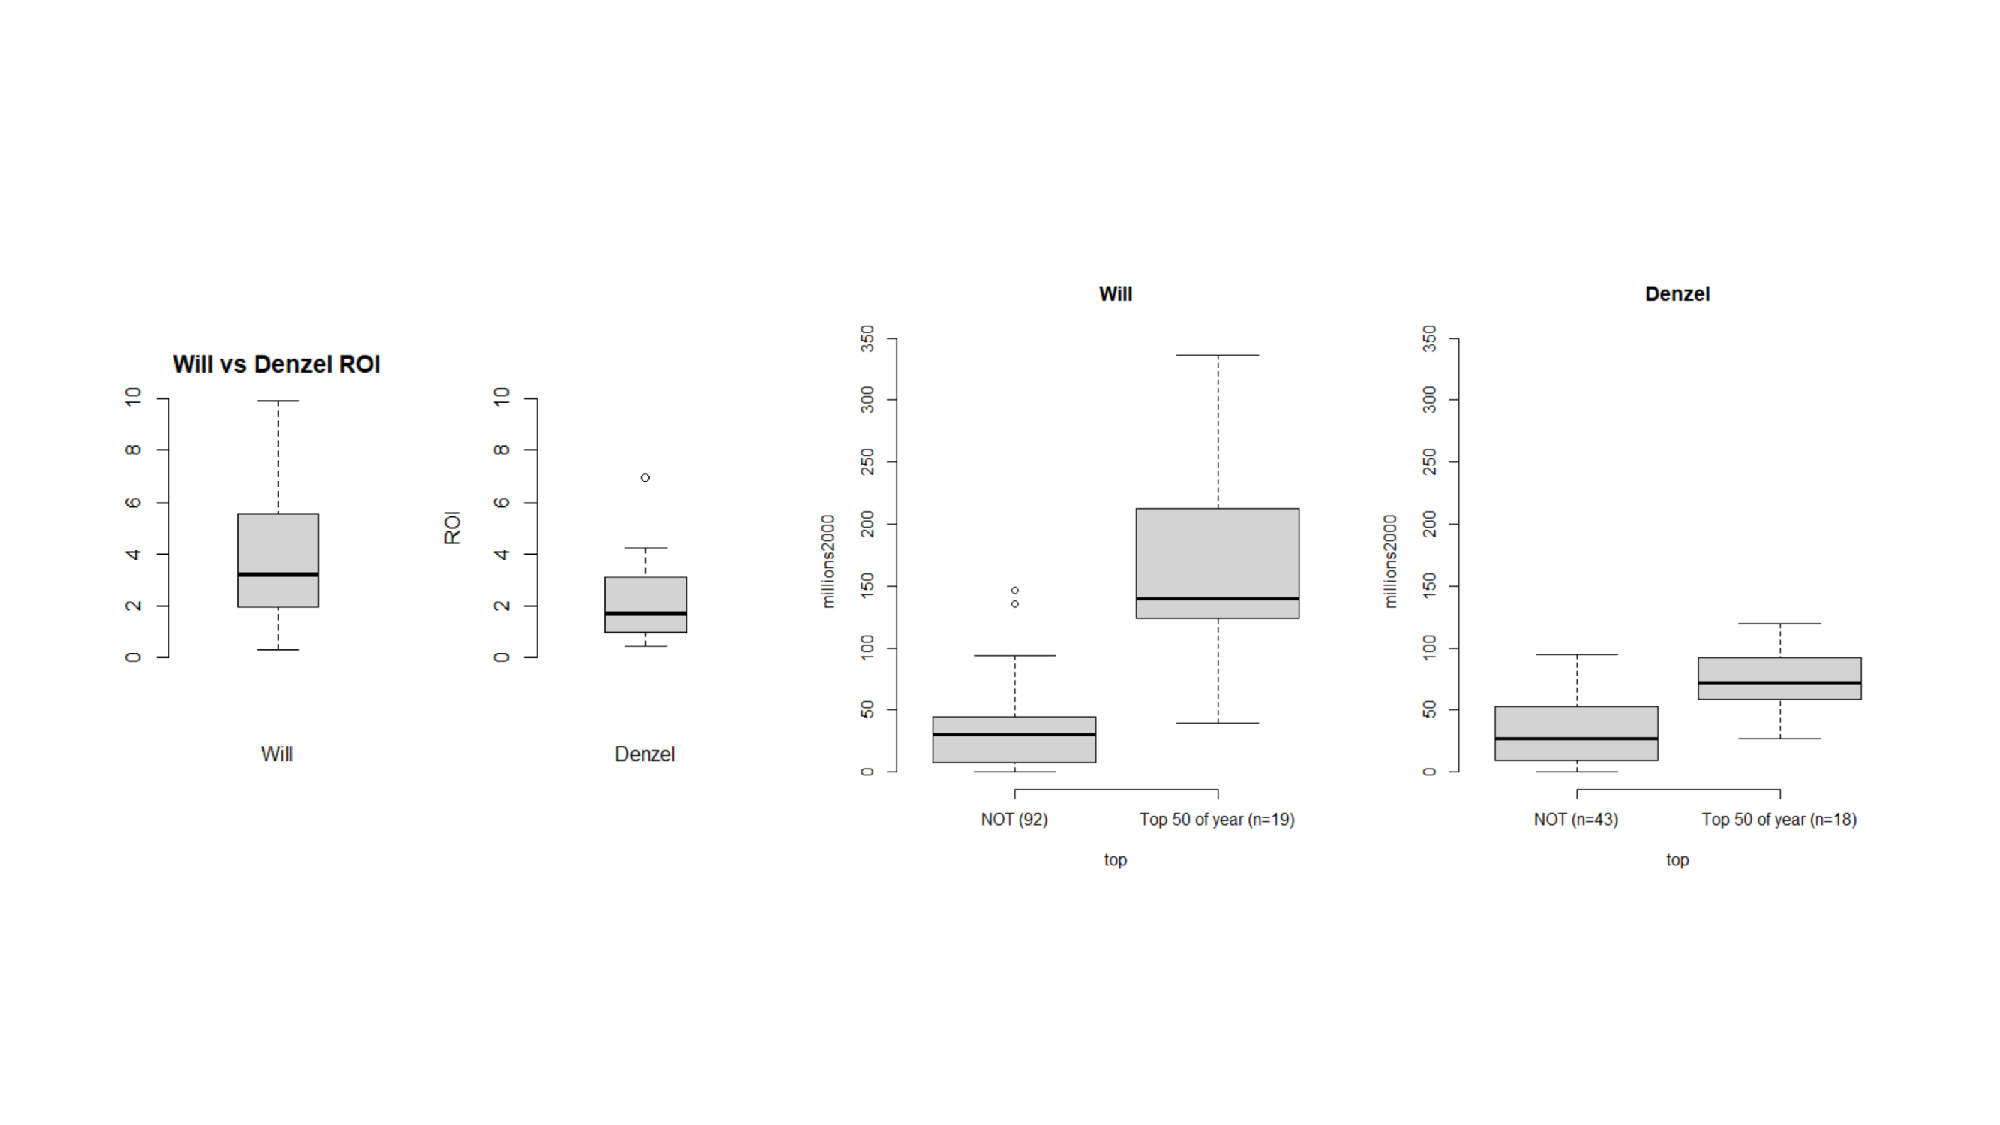
\includegraphics[trim = 0 0 0 0,clip,width=0.85\textwidth]{pdfs/oneimage.pdf} }
    \end{center}
    \label{fig:oneimage-1}
    \caption{ \textbf{One Image Description:} This shows Will and Denzels Return on Investment on the left and on the rights shows a boxplot of Will and Denzels top top movies income.}
    \hrule
\end{figure}

\section{Research Question:  What is my primary question}
\label{sec:rq}

Who is better, Will Smith or Denzel Washington?

\section{Data Description}
\label{sec:data}

This data was scraped from the IMDB website by Monte Shaffer in the Fall
semester of 2020. It is 50Mb and contains about 10,000 movies with their
movie rank, year, title, genre, rated, rating, minutes, metacritic,
votes, millions, paragraph, country, language, release date, budget, and
productions companies. From there this data was narrowed into the top
2000 movies. Where I looked into Will Smiths movies and Denzel
Washington movies to examine deeper into who is really better? Parts of
my analysis were done with the whole data set but will be pointed out
when that is the case and when I use the top2000 movies.

\subsection{Summary of Sample}
\label{sec:data-sample}

This sample of data I used observes many things from the IMDB website.
The year, budget, title, profits, ratings, actors, metacritics, and
ranks of movies/actors.

\subsection{Summary Statistics of Data}
\label{sec:data-summary}

For the summary of statistics I used boxplots, plots, and some t test to
confirm relationships between Will and Denzel. I looked at boxplots of
ratings, metacritics, and ROI. I used plots to observe money and I ran a
couple t test to back my findings between boxplots.

\section{Key Findings}
\label{sec:findings}

\begin{figure}[!ht]
    \hrule
    \begin{center}
        \scalebox{1.00}{    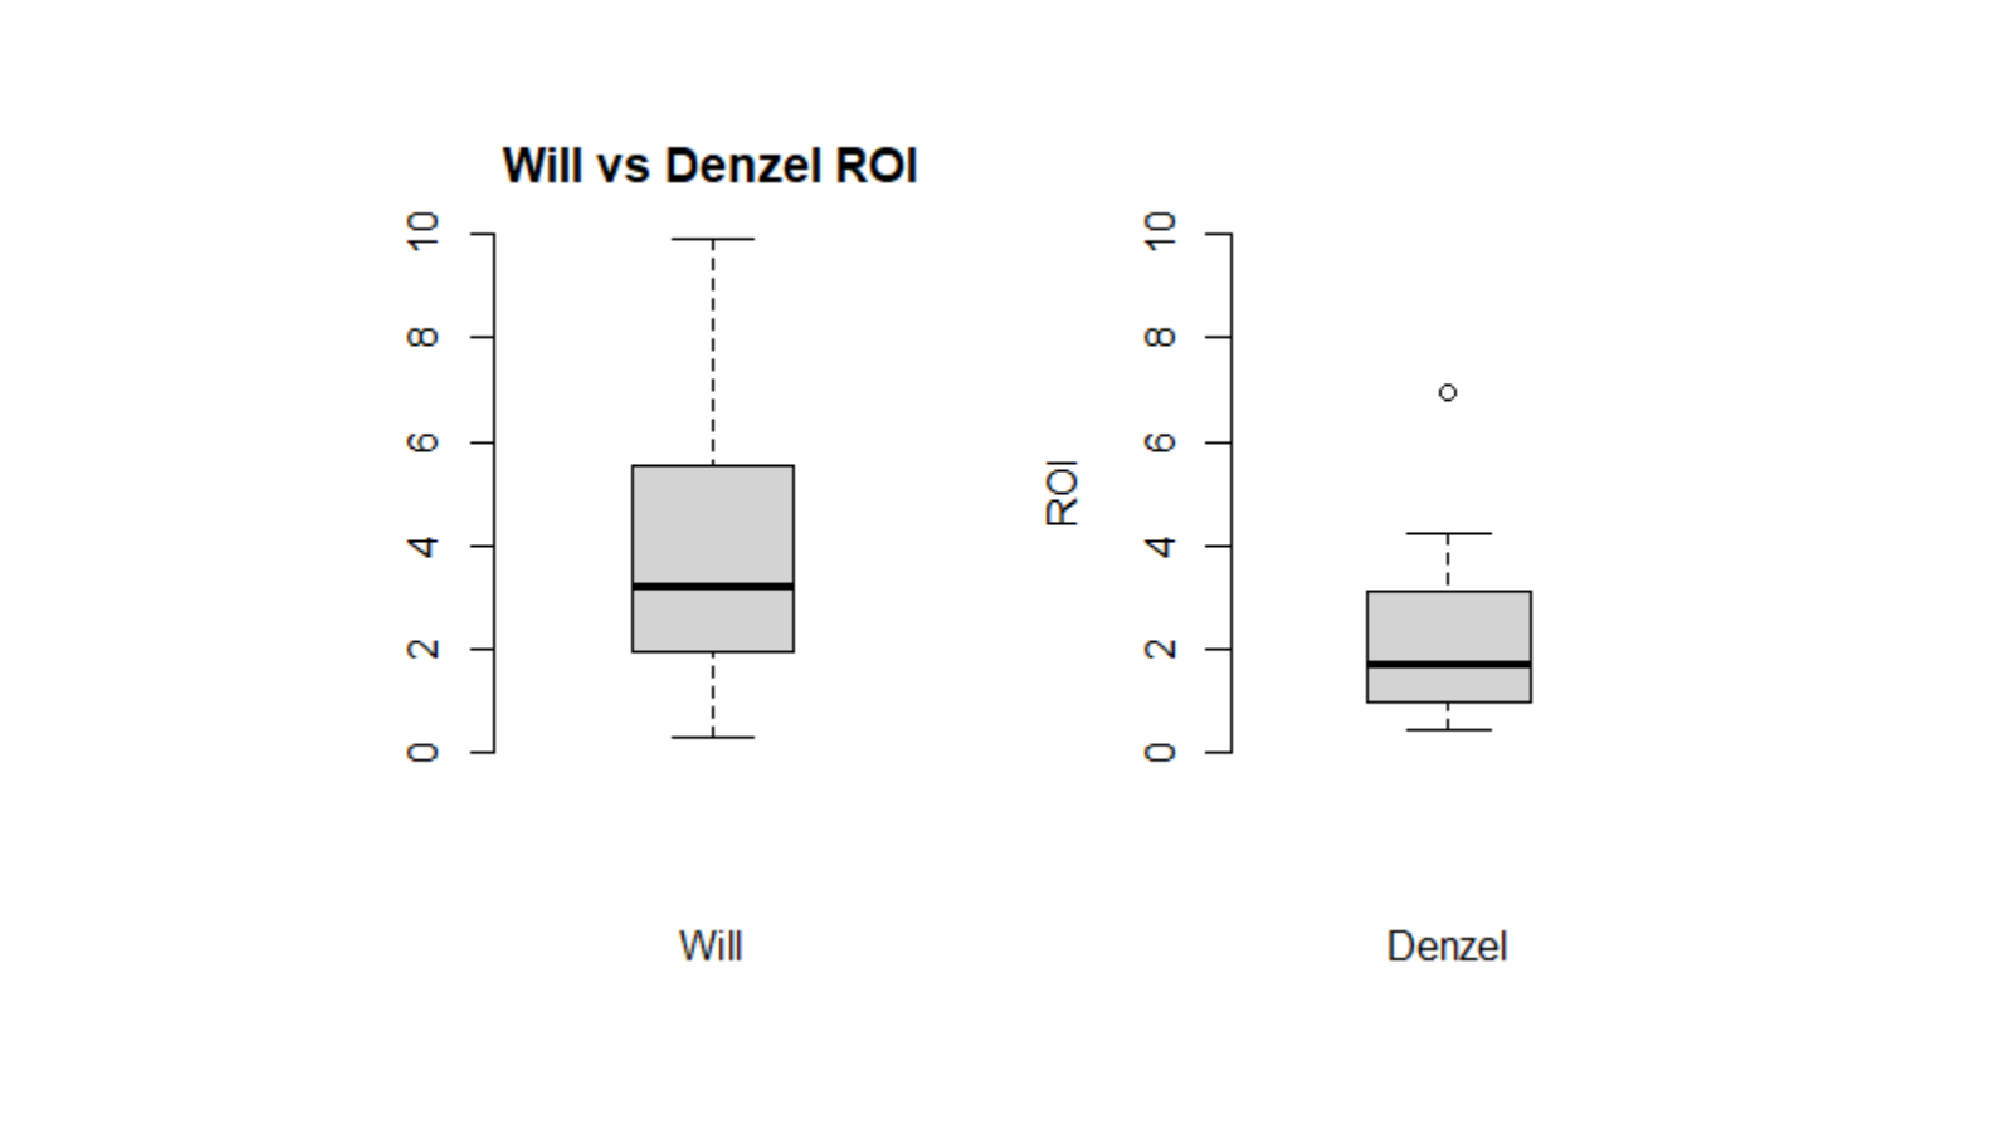
\includegraphics[trim = 0 0 0 0,clip,width=0.85\textwidth]{pdfs/ROI.pdf} }
    \end{center}
    \label{fig:oneimage-1}
    \caption{ \textbf{Return on investment:} This represents Will (on the left) and Denzels (on the right) return on investment.}
    \hrule
\end{figure}

Return on investment represents the financial benefit from an
investment. This was calculated by taking the net benefits of movies and
dividing by the total cost. I felt as the ROI could explain a lot. So I
decided to look into how much Will and Denzel were making on these
investments. I chose to look into the top 2000 movies and of those
movies, Will has 19 movies in the top 2000 and Denzel has 18 in the top
2000 movies. Of those I found overall Will has a higher ROI by quite a
bit. This some what makes sense as Will has preformed more overall
movies and he also has his foot in the door in Hollywood. This makes me
wonder, is there money laundering going on? Or do some movies just
happen to catch society attention more than others? I also found that
Will has a larger budget to spend so that I think is a big factor to why
he gets a bigger return. Wills budget on average was 100 million whereas
Denzels was closer to 45 million, so about half. With that, I don't
think it is fair to say that an ROI is a deciding factor on if someone
is better than the other. Yet, I think it shows that Will Smith may be a
better movie star but not necessarily a better person. I think this also
has influence to show that Will Smith does play in more movies or has
some shady business going on because can still be a movie star making a
lot of movie and be a bad person.

\begin{figure}[!ht]
    \hrule
    \begin{center}
        \scalebox{1.00}{    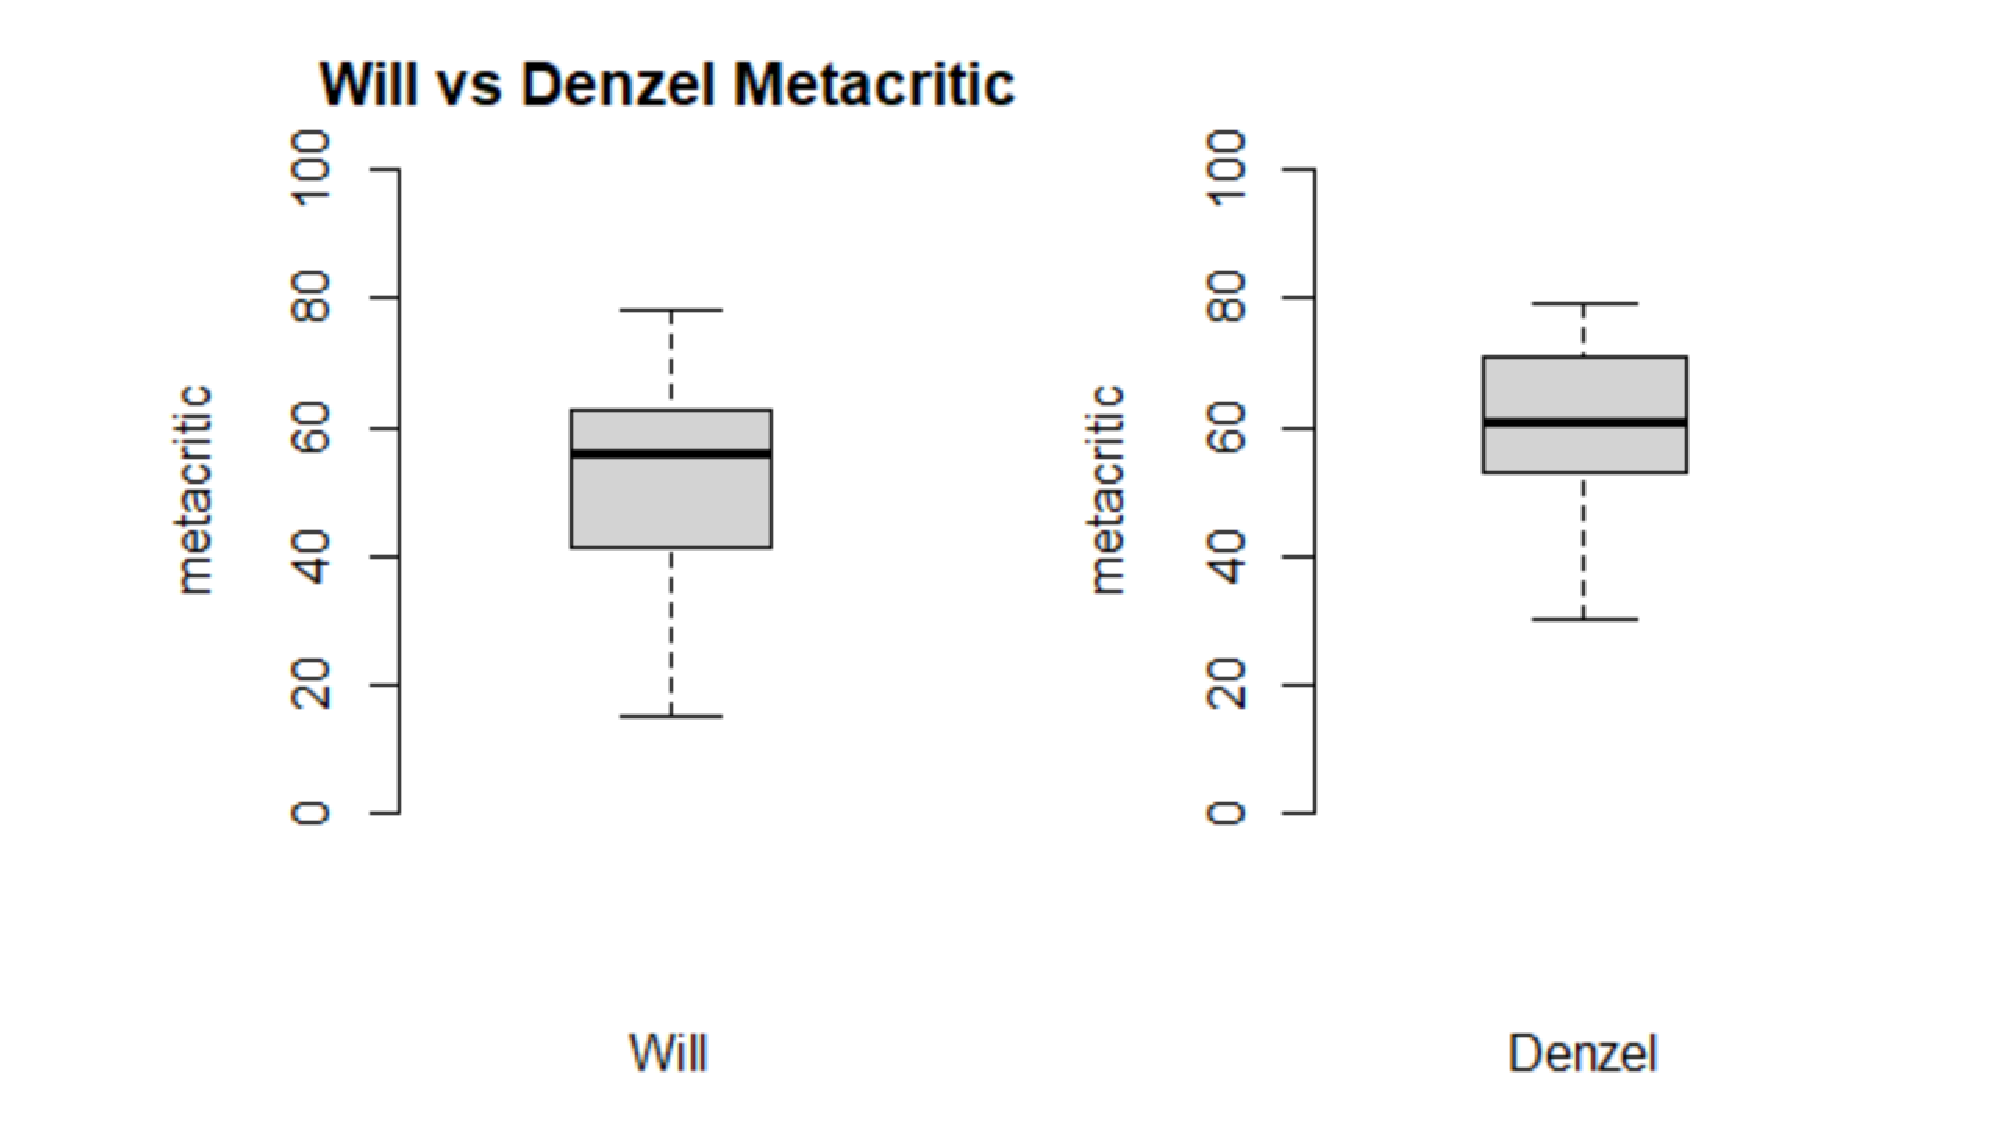
\includegraphics[trim = 0 0 0 0,clip,width=0.85\textwidth]{pdfs/metacritic.pdf} }
    \end{center}
    \label{fig:oneimage-1}
    \caption{ \textbf{Metacritic:} This represents the ratings of Metacritic.}
    \hrule
\end{figure}

Metacritic is a website that generates reviews on films, TV shows,
music, and much more. Those ratings being weighted scores. For these the
website scrapes the web to find movie critics and sum those ratings.
Metacritic is a reliable source that has links to all sources to prove
where the ratings are coming from. With that I felt like this would be a
huge telling on who is better. So I used the whole data set and not just
the top2000 movies. I then went on plot the metacritic ratings to see
who scored higher and you can see that Denzel's ratings are higher
overall and on average.

\newpage

\begin{figure}[!ht]
    \hrule
    \begin{center}
        \scalebox{1.00}{    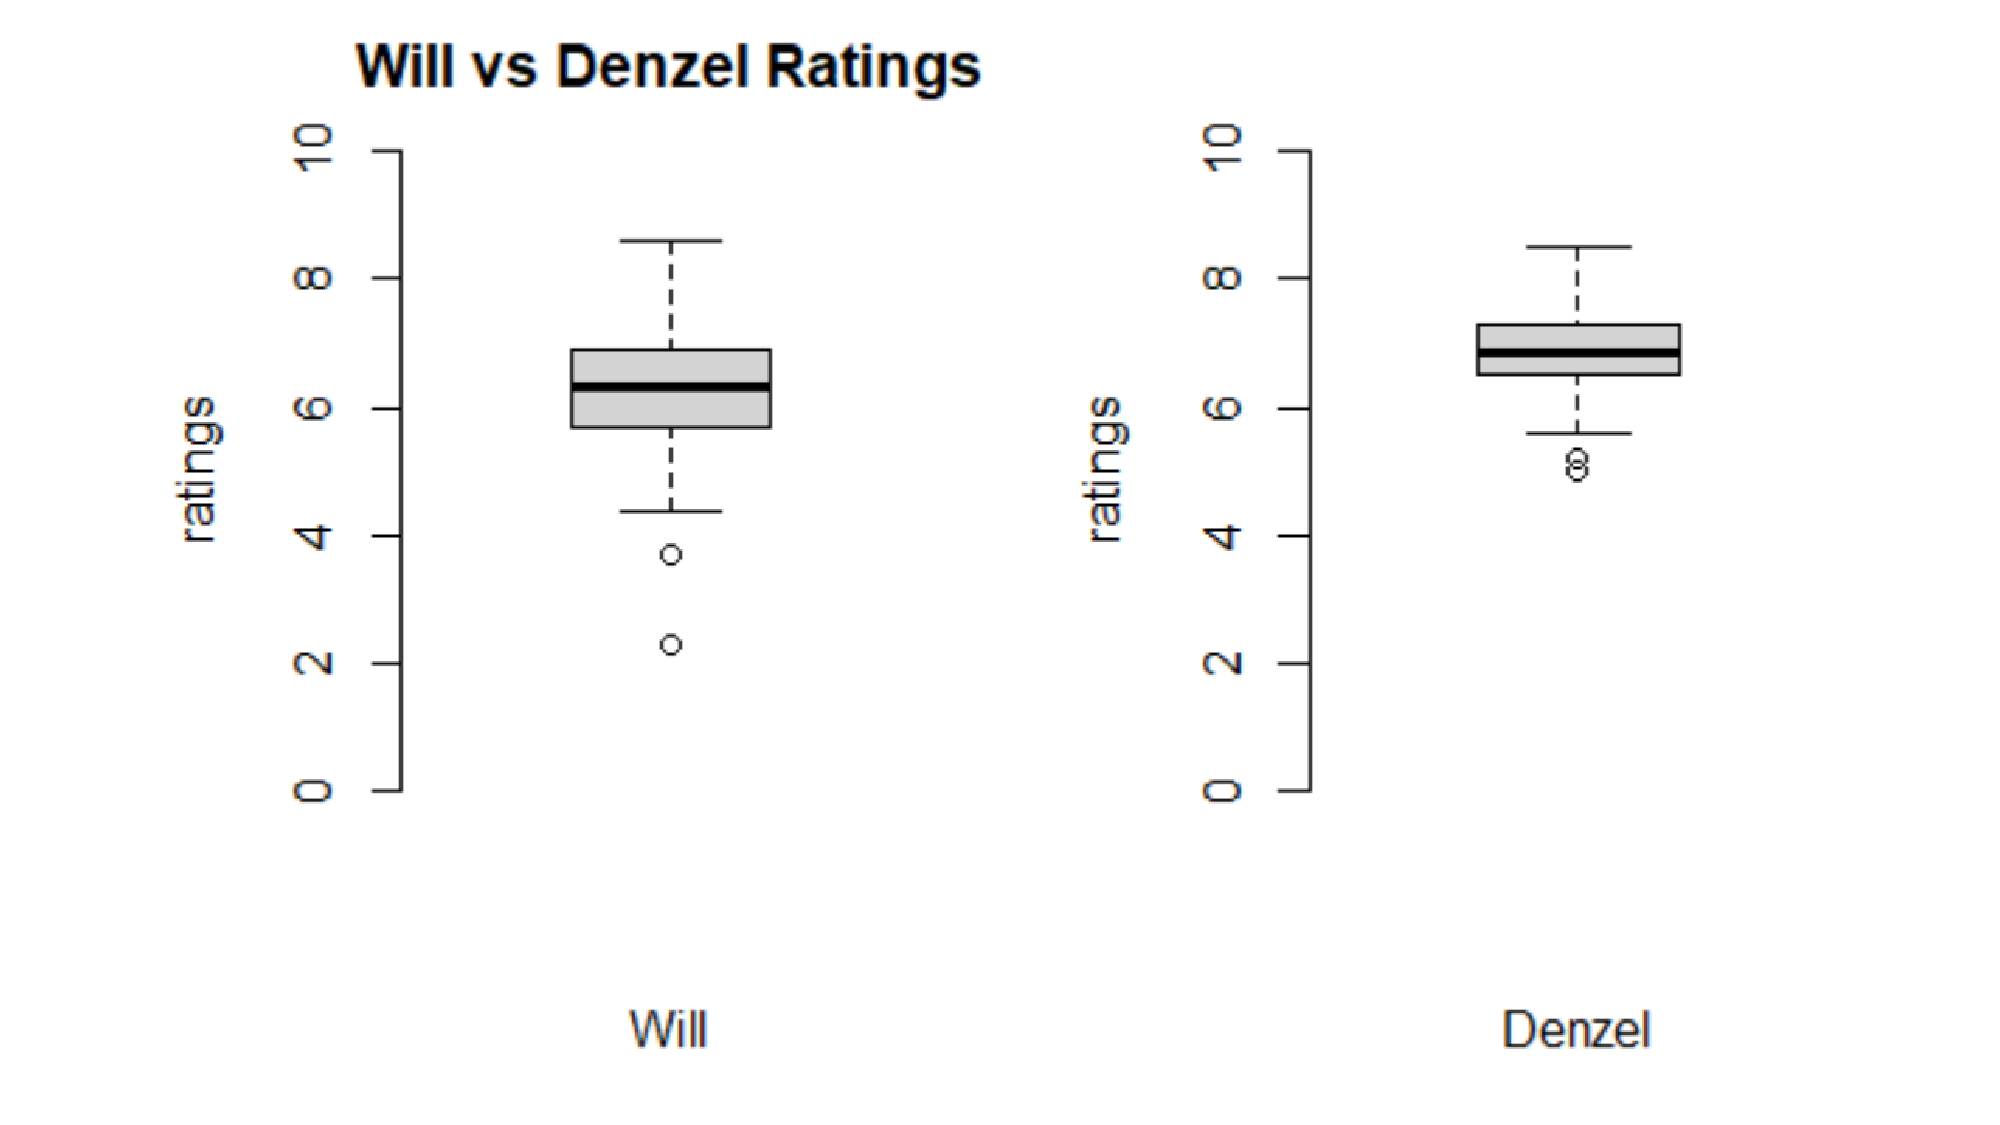
\includegraphics[trim = 0 0 0 0,clip,width=0.85\textwidth]{pdfs/ratings.pdf} }
    \end{center}
    \label{fig:oneimage-1}
    \caption{ \textbf{Ratings:} This represents the ratings from IMDB.}
    \hrule
\end{figure}

These rating represent the IMDB rating. This is on a scale of 1-10 and
from this you can see once again Denzel has a higher rating. Denzels
average rating is about 7 whereas Wills average rating is about 6. I
also found it interesting that Will has some outliars around 2 and 4
whereas Denzel does not. Thus, meaning that there were some people that
did not like Will or his movies.

\begin{figure}[!ht]
    \hrule
    \begin{center}
        \scalebox{1.00}{    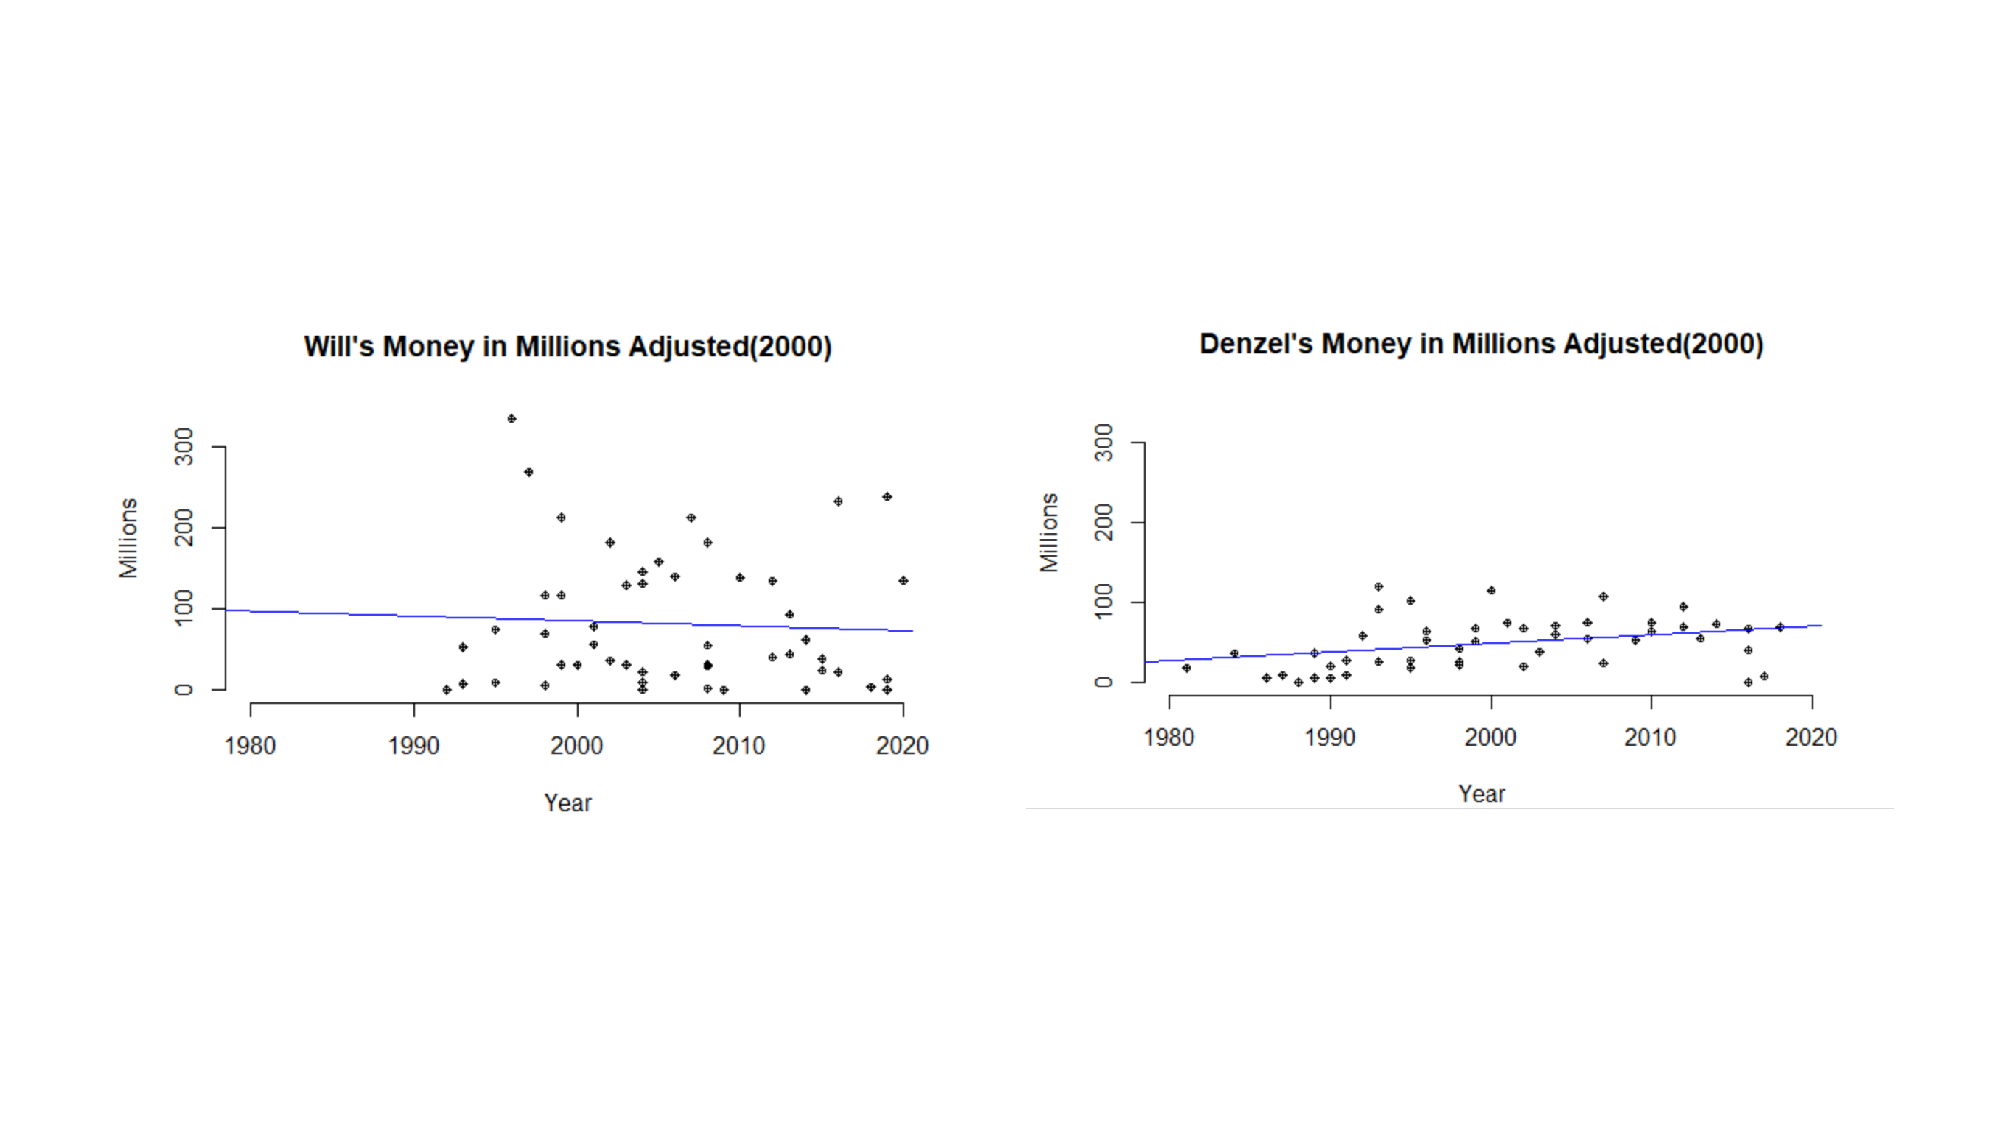
\includegraphics[trim = 0 0 0 0,clip,width=0.85\textwidth]{pdfs/money.pdf} }
    \end{center}
    \label{fig:oneimage-1}
    \caption{ \textbf{Money:} This represents the money made.}
    \hrule
\end{figure}

This observations was done over the the popular movies as I was curious
after looking into the ROI, how much money Will and Denzel were making?
Looking at all my data I focused on it after it was inflated to the year
2000. I found it interesting that Will's money is decreasing throughout
his career, meaning that he has made less throughout the years. Whereas
Denzel shows an increase in slope meaning throughout his career he has
had made an increase in money.

\section{Conclusion}
\label{sec:conclusion}

Will has larger movie budget then Denzel so in my opinion he should make
more money and have a bigger ROI. But just cause you make more money
does not make you better. Being better then someone is very vague but is
not defined by income as much as it does influence. Those who are
influential to the community and those around them are better people
than those who don't. Thus, I think the metacritic and ratings have a
bigger influence on deciding whether someone was a good actor. Plus, the
data shows Denzel is ranked higher as an actor, as well as for
metacritic votes. This leads me to believe that Denzel may be the better
actor. Those who make a lot of money in Hollywood could be a great movie
star and still be hated by many. Therefore, not a ``better'' person
because we all know that money can influence the good, bad, and ugly.
Overall, I think its fair to say money does not define a good or bad
person but ranks and ratings give a more precise representation of who
the better person is.

Lastly, I think it is interesting that Will's money made has been
steadily decreasing. Where Denzels continues to grow. I think that this
could be that Denzel is picky about who he does his movies with unlike
Will who may take any movie, good or bad. Which makes me think that this
may be another reason that Will has a lower ratings. He will take and do
any movie if it is good or bad whereas Denzel appears to pick and choose
wisely. With that I conclude that Denzel Washington is a overall better
actor than Will Smith.




%% appendices go here!


\newpage
\theendnotes

%%%%%%%%%%%%%%%%%%%%%%%%%%%%%%%%%%%  biblio %%%%%%%%
\newpage
\begin{auxmulticols}{2}
\singlespacing 
\bibliography{./../biblio/master.bib}

%%%%%%%%%%%%%%%%%%%%%%%%%%%%%%%%%%%  biblio %%%%%%%%
\end{auxmulticols}

\newpage
{
\hypersetup{linkcolor=black}
\setcounter{tocdepth}{3}
\tableofcontents
}



\end{document}